\chapter{Eksperymenty}

W niniejszym rozdziale przedstawiony został krótki opis środowiska testowego oraz przebieg testów układu do zmiany przełożeń.

\section{Środowisko testowe}
Wszystkie eksperymenty przeprowadzone zostały w sposób stacjonarny. Zamontowanie roweru na dedykowanym stojaku umożliwia swobodną symulację dowolnych scenariuszy testowych. Akwizcyja danych sterownika układu jest w takim przypadku zdecydowanie mniej problematyczna, ponieważ nie jest konieczne stosowanie protokołów transmisji bezprzewdowej. 
Na potrzeby testów, wykonana została aplikacja przedstawiająca, w formie przebiegów czasowych, kluczowe parametry układu. Wykorzystano język C++ oraz zestaw bibliotek Qt. Komunikacja pomiędzy sterownikiem a aplikacją nawiązana została za pomocą intefrejsu szeregowego UART(ang. \textit{Universal Asynchronous Receiver and Transmitter}). Sterownik pracujący w trybie testowania, wysyła zastaw danych do komputera PC z częstotliwością 20Hz. Zestaw danych, składa się z chwilowych wartości:
\begin{itemize}
 \item
 kąta nachylenia podłoża,
 \item
 kadencji,
 \item
 prędkości liniowej roweru,
 \item
 wybranego biegu,
 \item
 stanu przycisku redukującego przełożenie,
 \item
 stanu przycisku zwiększającego przełożenie,
 \item
 trybu pracy sterownia.
 \end{itemize}
 
We wszystkich trybach automatycznych przedstawione są również przyjęte zakresy kadencji, a w trybie sportowym dodatkowo zakres kąta nachylenia podłoża.
 
\section{Wyniki tesów}

Poniżej zaprezentowano wyniki testów wybranych scenariuszy, potwierdzające zgodność działania sterownika układu z założeniami, przedstawionymi w pkt. \textcolor{red}{pktFinalny}
\subsection{Tryb ręczny}
Podstawowa funkcjonalność układu to zmiana przełożeń w trybie ręcznym. Naciśnięcie odpowiedniego przycisku powoduje zmianę przełożenia.
 
\begin{figure}[h]
    \centering
    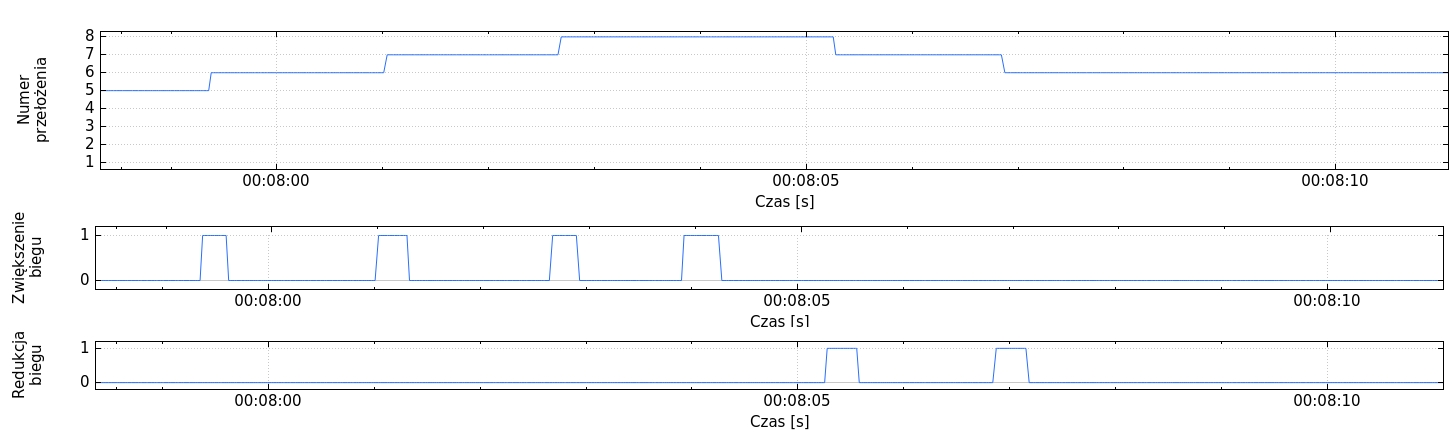
\includegraphics[scale=0.36]{tests_randomChange1.jpg}
    \caption{Zmiana przełożeń w trybie ręcznym}
    \label{fig:tests_randomChange}
\end{figure}

Kolejna funkcjonalność to możliwość zmiany kilku przełożeń w wyniku naciśniecia i przytrzymania odpowiedniego przycisku. Funkcjonalność ciągłej zmiany przełożeń zaprojektowana została z myślą o możliwości szybkiego doboru przełożenia. Początkowo zakładano, że zmiana biegów wyzwalana będzie z częstotliwością 1Hz. Jednak w trakcie przeprowadzania eksperymentów uznano, że należy zmniejszyć opóźnienie pomiędzy kolejnymi zmianami, które ostatecznie wynosi 0.7 sekundy.

\begin{figure}[h]
    \centering
    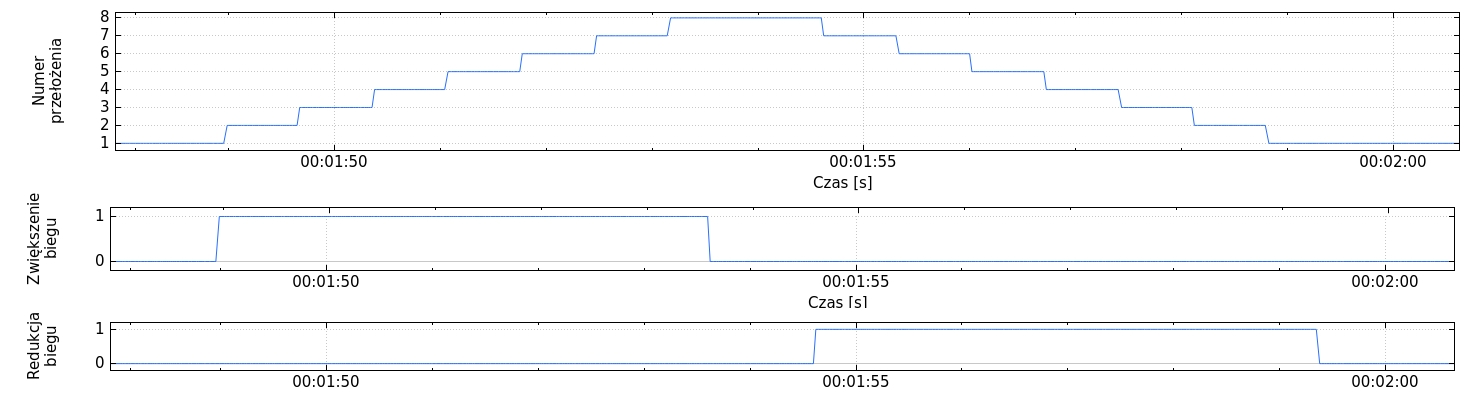
\includegraphics[scale=0.36]{tests_continousChange.jpg}
    \caption{Ciągła zmiana przełożeń w trybie ręcznym}
    \label{fig:tests_continousChange}
\end{figure}
\subsection{Tryb comfort}
W trybie comfort zweryfikowano dwa scenariusze testowe. 

Pierwsza przetestowana funkcjonalność to utrzymywanie kadencji w zadanym zakresie. W trybie comfort kadencja powinna zostać utrzymana w zakresie od $45$ do $60$ obrotów na minutę. Szare linie naniesione na wykres kadencji obejmują ten zakres. Przebiegi zamieszczone na rys. \ref{fig:tests_continousChange} potwierdzają poprawne działanie tej funkcjonalności. W wyniku przekroczenia górnej granicy wartości kadencji następuje automatyczna zmiana przełożenia. Stan przycisków do zmiany ręcznej nie zmienia się. Przełożenie zmieniane jest dwukrotnie. Kolejne zmiany przełożeń nie są konieczne w wyniku stabilizacji wartości kadencji w zadanym zakresie. 
\begin{figure}[h]
    \centering
    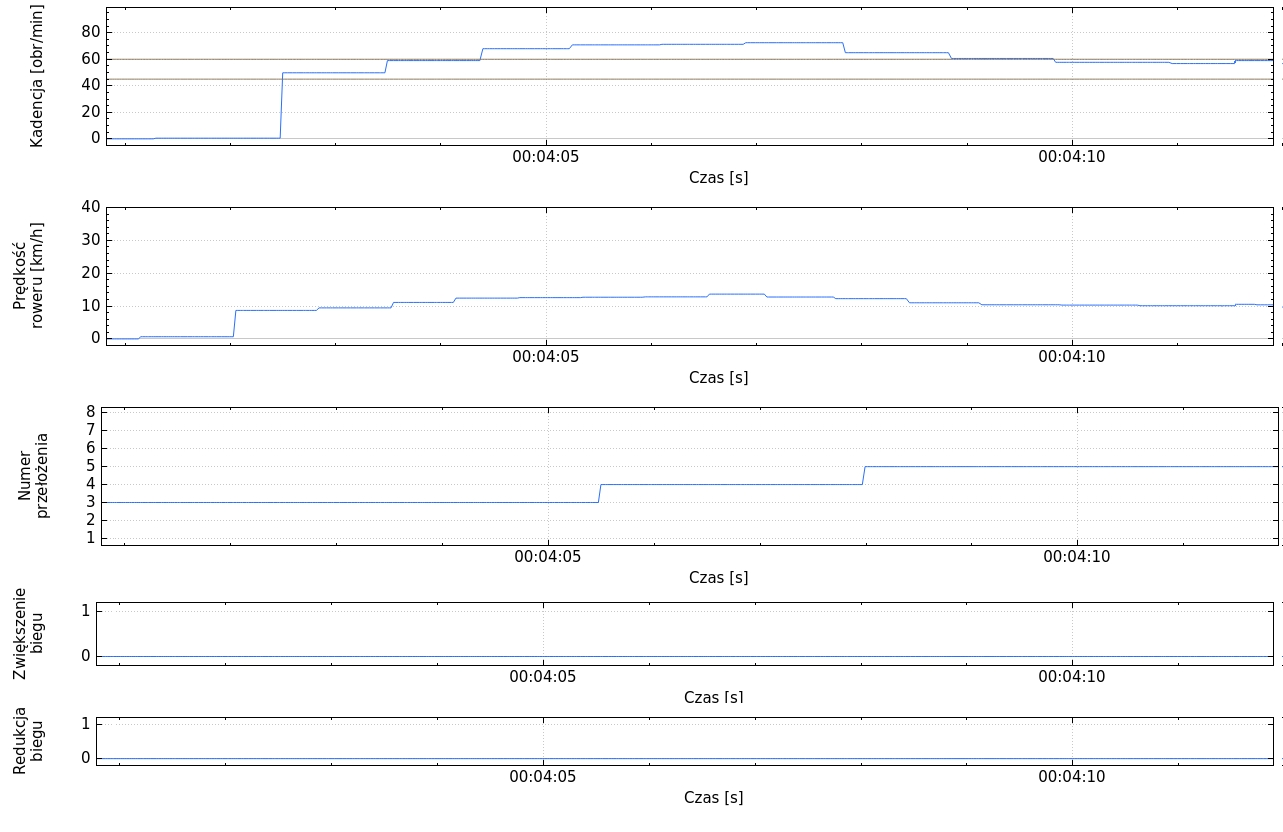
\includegraphics[scale=0.36]{tests_trybComfort.jpg}
    \caption{Automatyczna zmiana przełożeń - tryb Comfort.}
    \label{fig:tests_trybComfort}
\end{figure}

Drugi scenariusz obejmuje sprawdzenie wyłączenia możłiwości ręcznej zmiany przełożeń. Przebiegi przedstawione na rys. \textcolor{red}{RYS!} potwierdzają poprawne działanie kontrolera. Przełożenie jest stałe pomimo zarejestrowanych prób ręcznej zmiany biegu.
\begin{figure}[h]
    \centering
    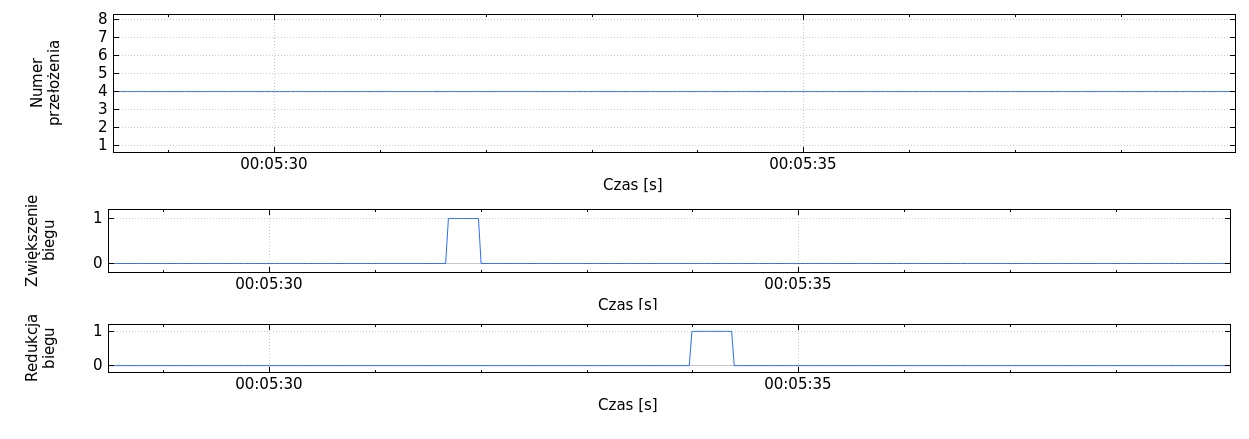
\includegraphics[scale=0.38]{tests_trybComfortBrakZmian.jpg}
    \caption{Brak reakcji na ręczną zmianę w trybie Comfort.}
    \label{fig:tests_noChange}
\end{figure}

\subsection{Tryb active}

Tryb active powinien zapewniać dwie funkcjonalności - utrzymanie kadencji w zadanym przedziale i ręczna zmiana biegów.

Zakres kadencji w trybie active wynosi od 55 do 70 obrotów na minutę. Na rys.\ref{fig:tests_active} można zaobserwować że kontroler dobiera  przełożenie tak, aby spełnić powyższe założenie.
\begin{figure}[h]
    \centering
    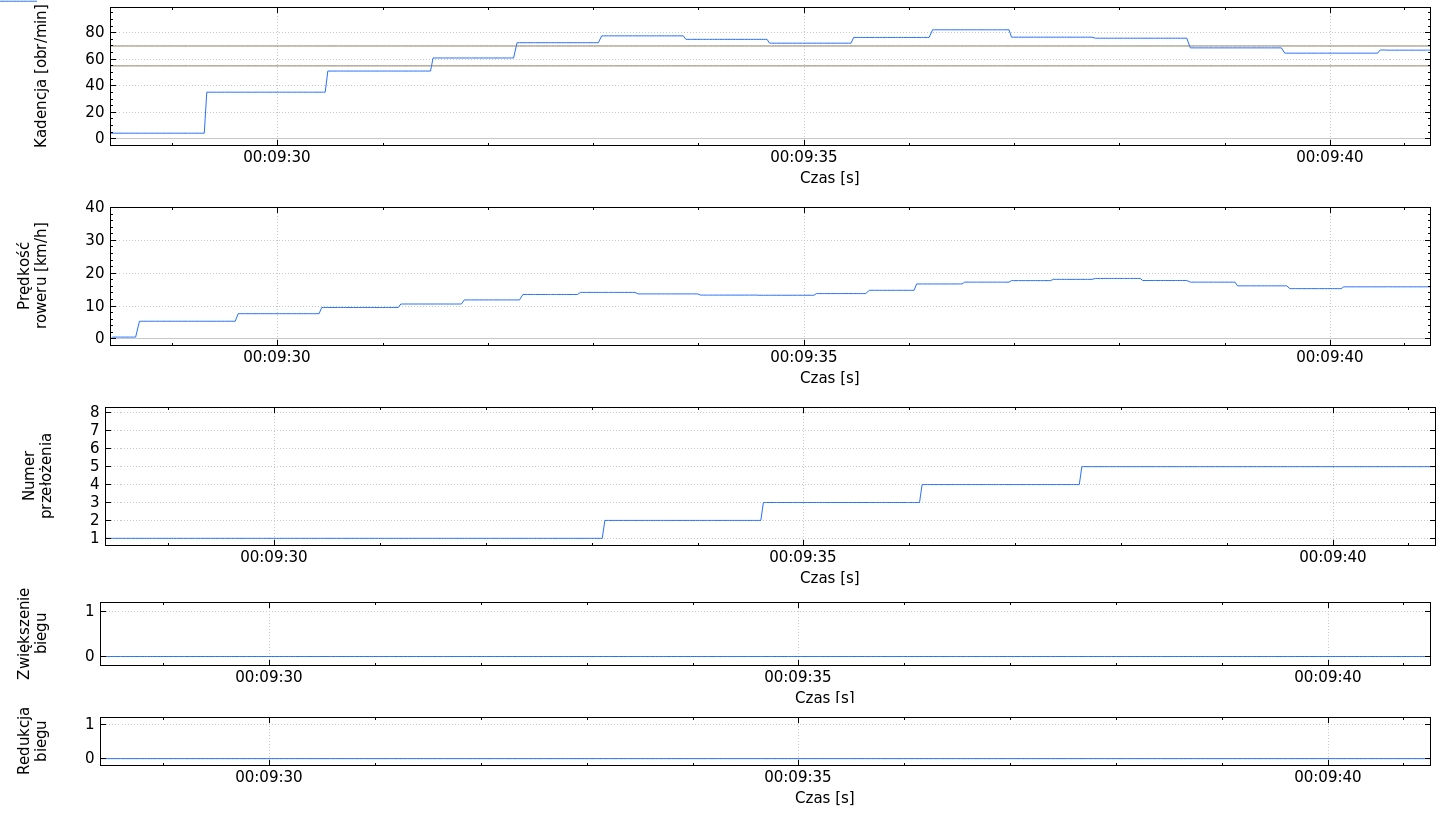
\includegraphics[scale=0.35]{tests_trybActive.jpg}
    \caption{Automatyczna zmiana przełożeń - tryb Active}
    \label{fig:tests_active}
\end{figure}

Kolejna funkcja dostępna w trybie active to ręczna zmiana przełożeń. W wyniku ręcznej zmiany przełożeń automatyczna zmiana biegów zostaje wyłączona na 10 sekund. Przebiegi zaprezentowane na rys. \ref{fig:tests_activeReczna} wykazują prawidłowe działanie sterownika. Ręczna zmiana biegu powoduje redukcje przełożenia, której konsekwencją jest wzrost wartości kadencji. Pomimo przekroczenia górnej granicy zakresu kadencji, zmiana biegu następuje dopiero po 10 sekundach.    
\begin{figure}[h]
    \centering
    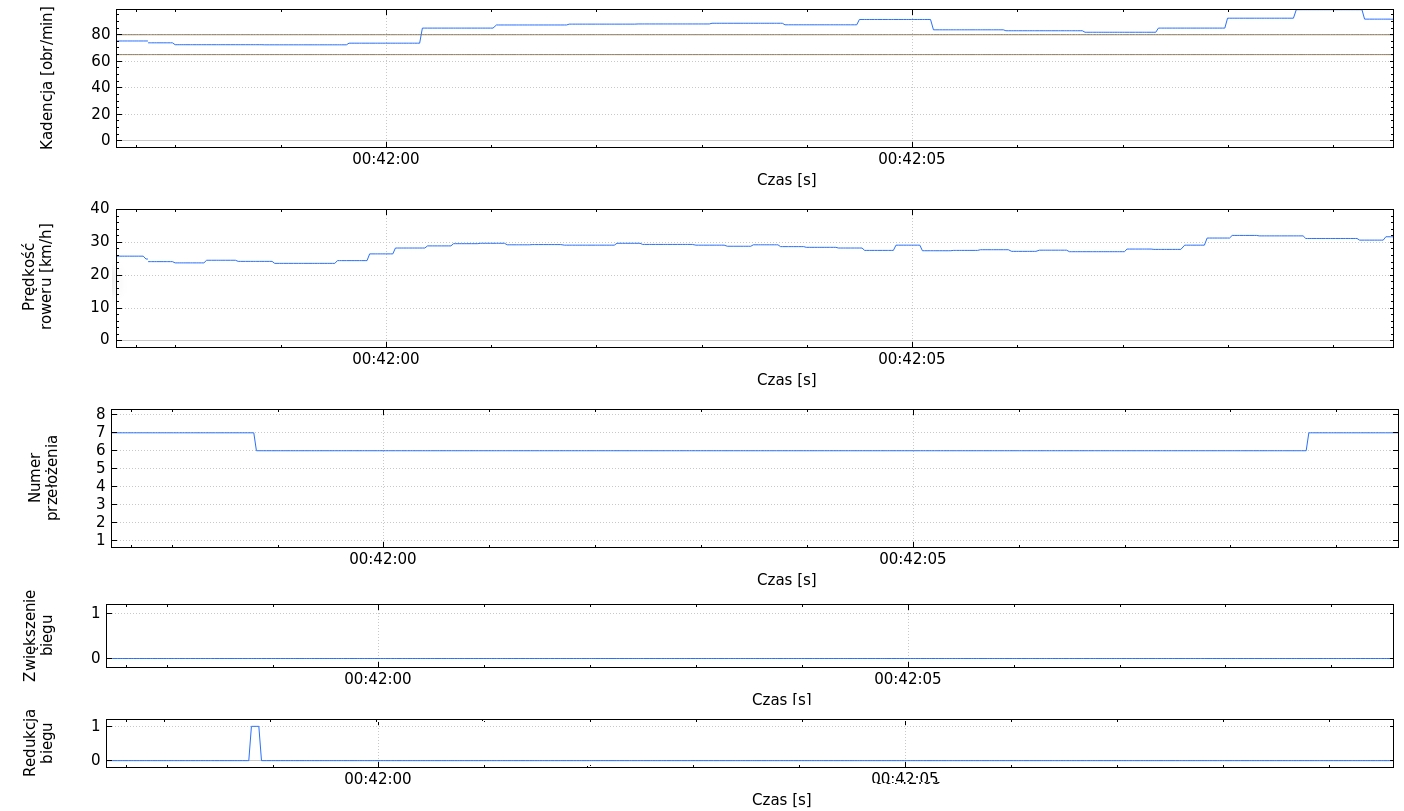
\includegraphics[scale=0.35]{tests_trybActiveRecznaZmiana.jpg}
    \caption{Automatyczna zmiana przełożeń - tryb Active}
    \label{fig:tests_activeReczna}
\end{figure}
\subsection{Tryb sport}
W trybie sportowym dokonywany jest odczyt danych pomiarowych z akcelerometru i żyroskopu. Zastosowanie filtru komplementarnego, który dokonuje fuzji tych danych, umożliwia wyznaczenie kąta nachylenia podłoża(pkt.\ref{kompZasadaDzialania}). Działanie filtru można dopasować poprzez dobór wartości stałej czasowej. Niska wartość stałej czasowej pozwala zachować niewielkie przesunięcie fazowe pomiędzy rzeczywistą wartością kąta nachylenia a wartością estymowaną. Jednoczesnie wartość estymowana obarczona jest błędem wynikającym z dryfu żyroskopu. Wysoka wartość stałej czasowej pozwala usunąć błędy wartości estymowanej, jednak wprowadza dodatkowe opóźnienie. Dobór tego parametru jest zależny od aplikacji.

Kąt nachylenia podłoża jest wielkością wolnozmienną, w porównaniu do np. kątów określających orientację wielowirnikowych platform latających. Niwelowanie błędu wynikającego z dryfu oraz przyspieszeń dynamicznych, działających na akcelerometr, ma wyższy priorytet, niż szybka odpowiedź filtru. Dlatego stała czasowa filtru powinna przyjąć wysoką wartość. Przebiegi przedstawione na rys.\ref{fig:tests_imu1} oraz \ref{fig:tests_imu2} przedstawiają estymowaną wartość kąta nachylenia podłoża dla przypadków, w których stała czasowa wynosi odpowiednio $0.5$ i $2$ sekundy. 
\begin{figure}[h]
    \centering
    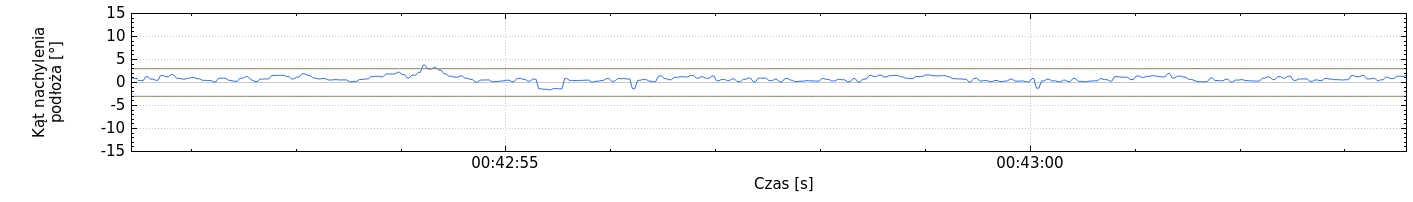
\includegraphics[scale=0.36]{tests_imu1.jpg}
    \caption{Automatyczna zmiana przełożeń - tryb Sport}
    \label{fig:tests_imu1}
\end{figure}

\begin{figure}[h]
    \centering
    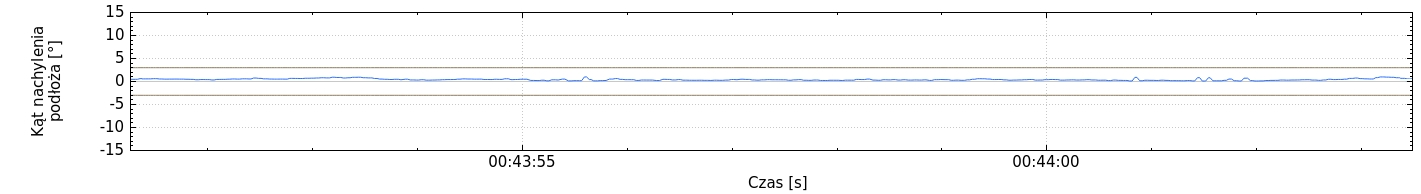
\includegraphics[scale=0.36]{tests_imu2.jpg}
    \caption{Automatyczna zmiana przełożeń - tryb Sport}
    \label{fig:tests_imu2}
\end{figure}
\begin{figure}[h]
    \centering
    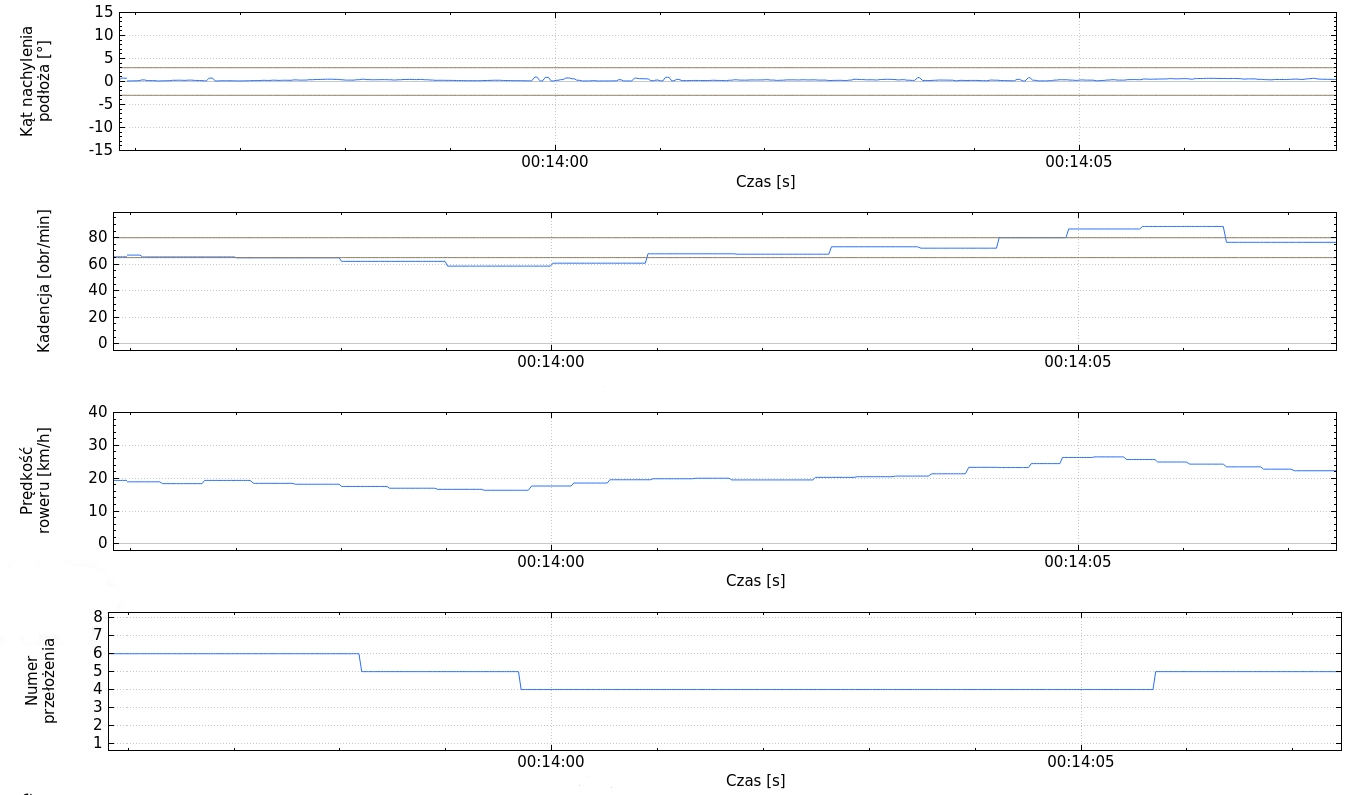
\includegraphics[scale=0.36]{tests_trybSportZmianaBiegow.jpg}
    \caption{Automatyczna zmiana przełożeń - tryb Sport}
    \label{fig:tests_sportMode}
\end{figure}

\begin{figure}[h]
    \centering
    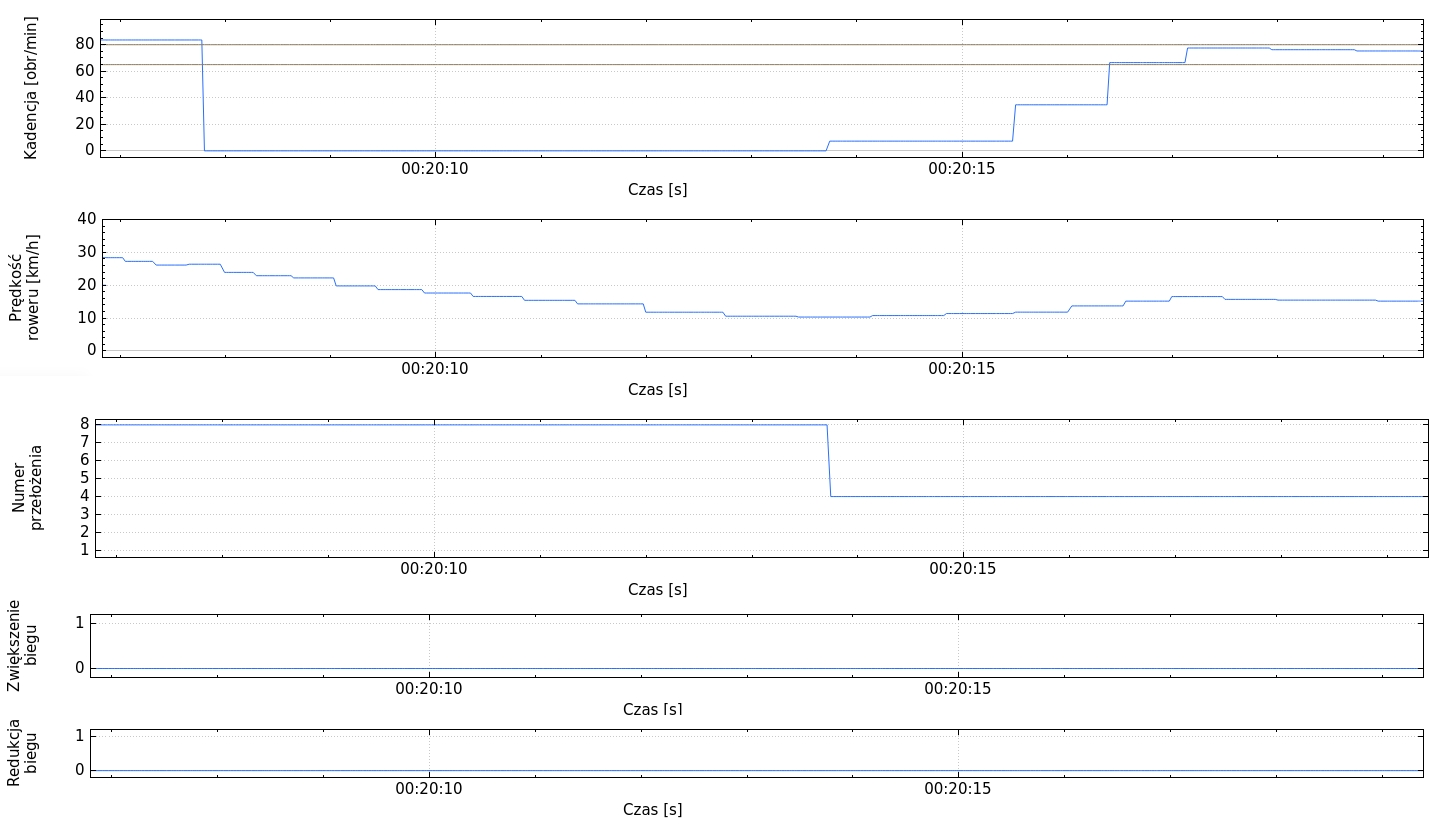
\includegraphics[scale=0.36]{tests_trybSportDopasowanieBiegu.jpg}
    \caption{Dopasowanie przełożenia w wyniku zatrzymania pedałowania - tryb Sport}
    \label{fig:tests_gearSpeedSelection}
\end{figure}




\begin{figure}[h]
    \centering
    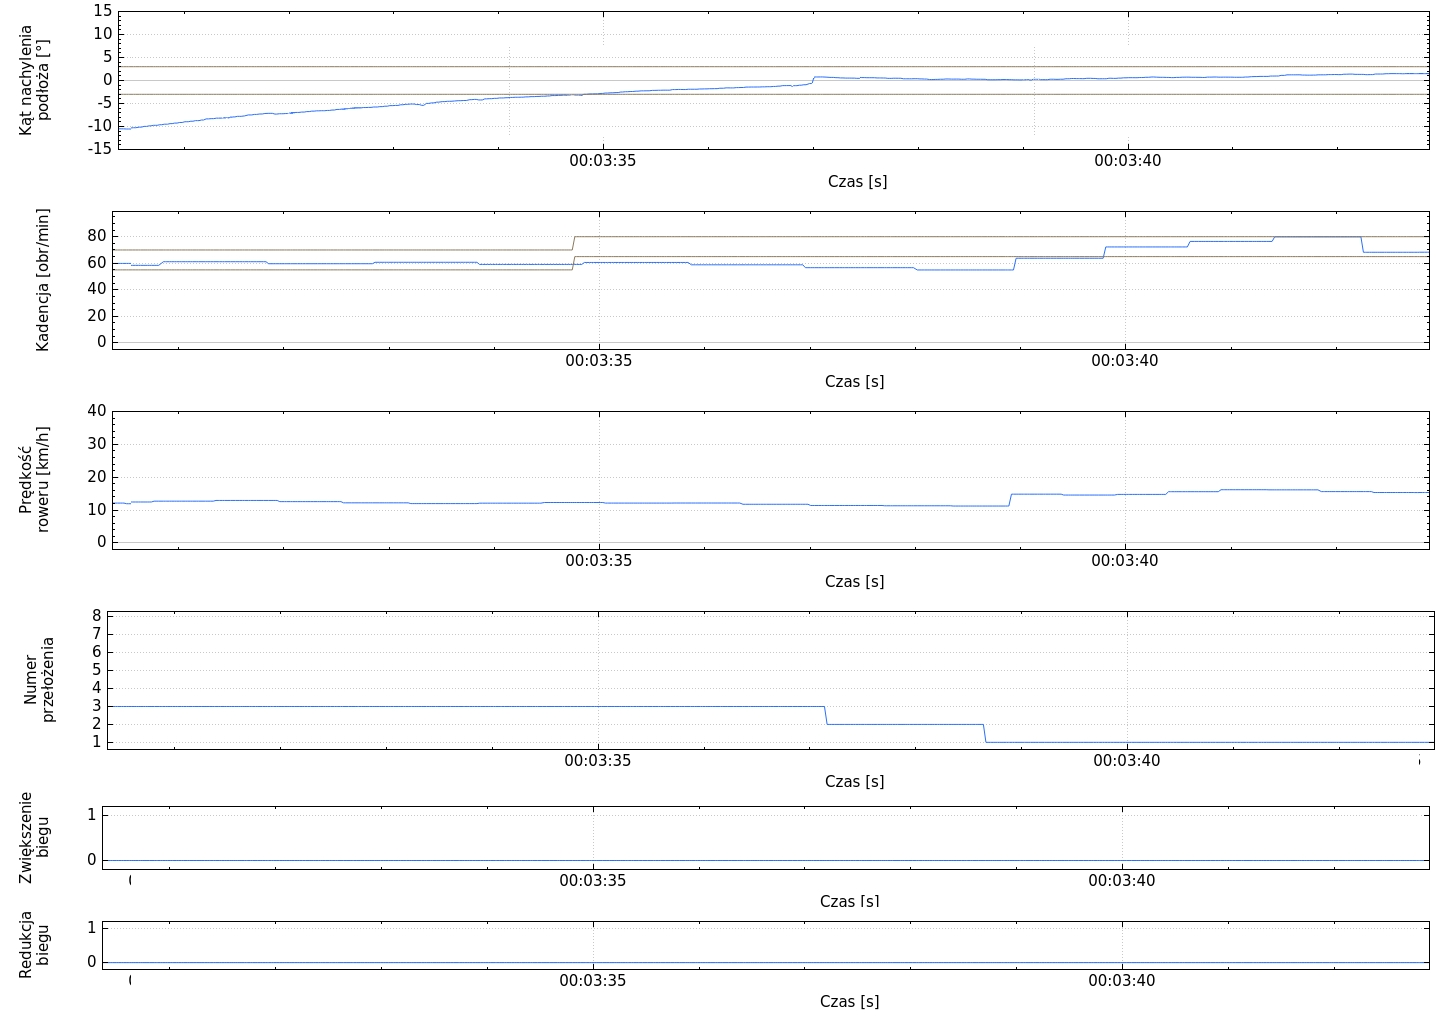
\includegraphics[scale=0.36]{tests_trybSportKat.jpg}
    \caption{Automatyczna zmiana przełożeń - tryb Sport}
    \label{fig:tests_sportMode}
\end{figure}

